\chapter{Imágenes de interés para el proyecto\label{apendA}}


\begin{figure}[htp]
\centering
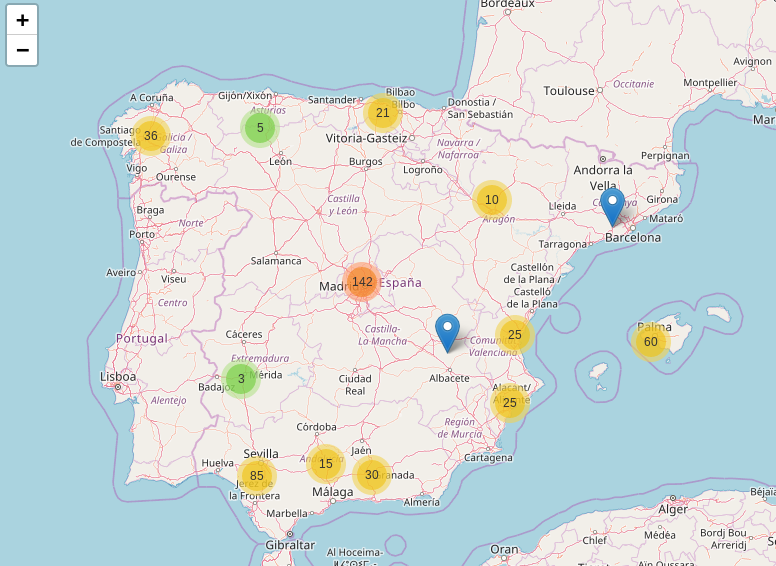
\includegraphics[scale=.50]{Anexos/PuntosNegrosEspana.png}
\caption{Puntos negros de España obtenidos.}
\label{blackShapes}
\end{figure}

\begin{figure}[htp]
\centering
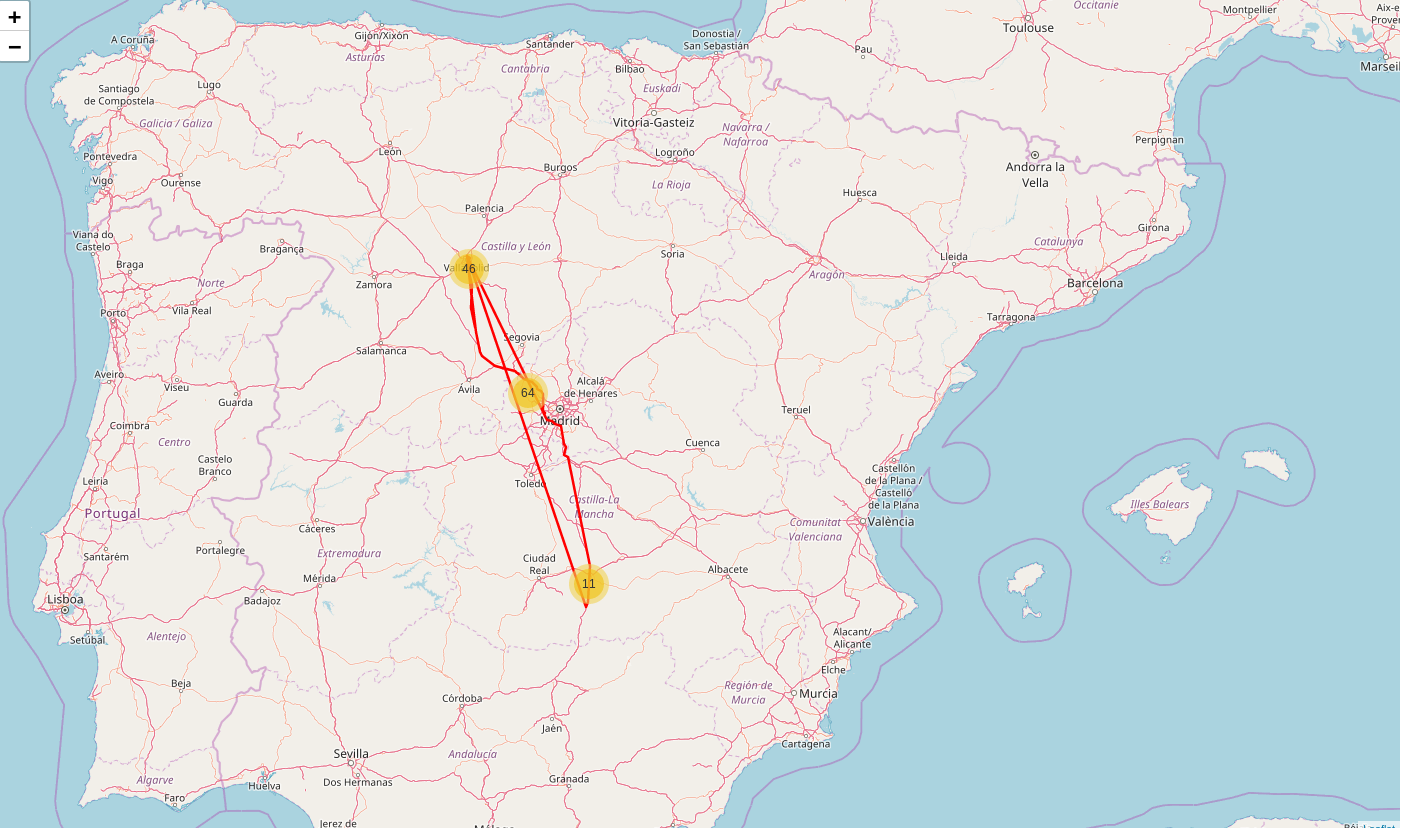
\includegraphics[scale=.30]{Anexos/rutaDeUnVehiculo.png}
\caption{Ruta de un vehiculo.}
\label{littleRoute}
\end{figure}


\begin{figure}[htp]
\centering
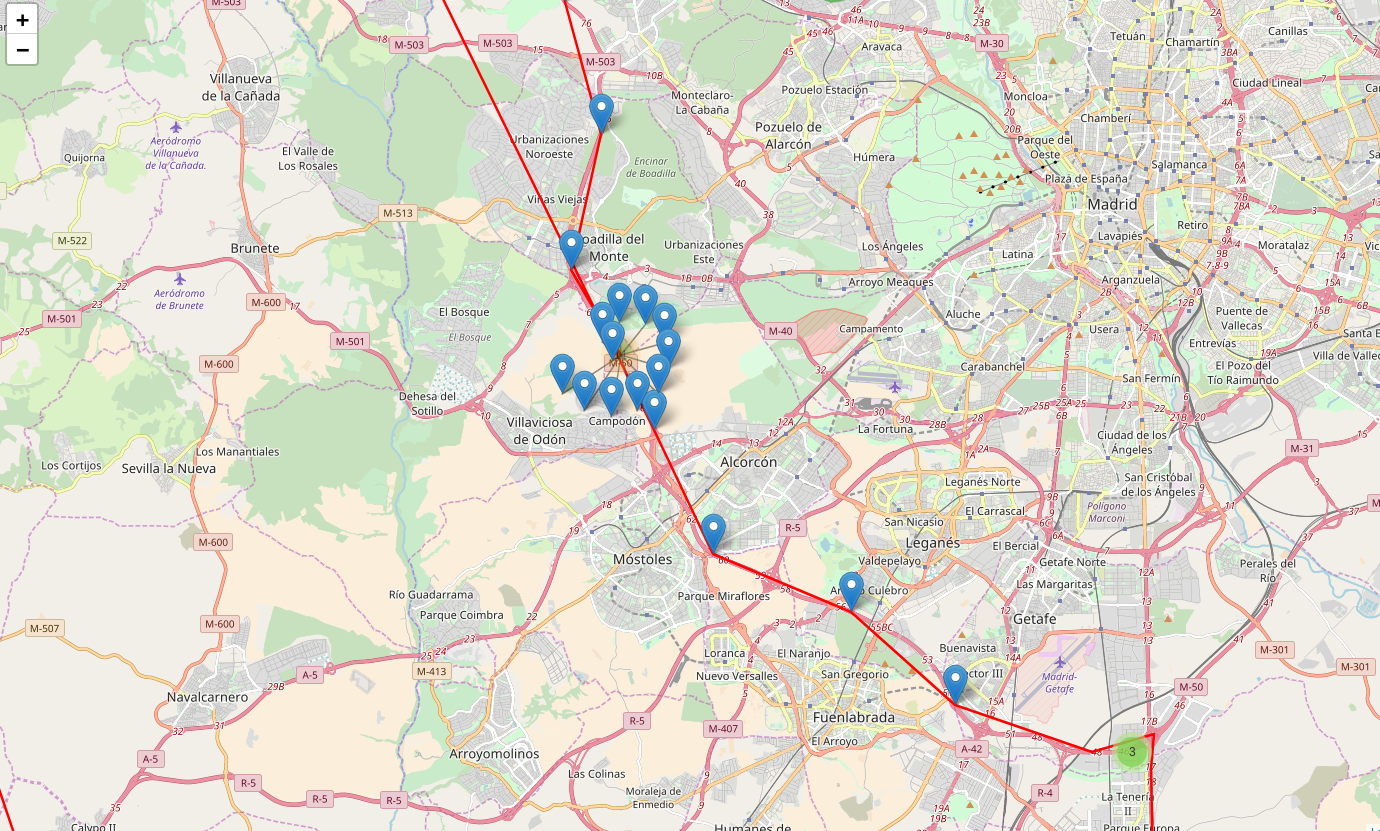
\includegraphics[scale=.30]{Anexos/rutaConParada.png}
\caption{Pequeña ruta y parada de un vehiculo.}
\label{littleRouteWithStop}
\end{figure}


\chapter{Script para el API de consultas a MongoDB integrado con OSM\label{apendB}}
\lstinputlisting[language=Python, basicstyle=\scriptsize]{Anexos/mongoUbicationServer.py}

\newpage
\chapter{Script de envio de tramas para la simulación\label{apendC}}
\lstinputlisting[language=Python, basicstyle=\scriptsize]{Anexos/sendTraffic.py}

\newpage
\chapter{Script de SparkSQL Streaming}\label{apendD}
\lstinputlisting[language=Python, basicstyle=\scriptsize]{Anexos/sparkStructStream.py}

\newpage
\chapter{Script de Spark Streaming}\label{apendE}
\lstinputlisting[language=Python, basicstyle=\scriptsize]{Anexos/sparkStreamingWithoutMongo.py}

\newpage
\chapter{Script de SparkSQL Streaming con las consultas a MongoDB}\label{apendF}
\lstinputlisting[language=Python, basicstyle=\scriptsize]{Anexos/sparkStreaming.py}

\newpage
\chapter{Script de creación del índice en Elasticserach}\label{apendG}
\lstinputlisting[language=Python, basicstyle=\scriptsize]{Anexos/CreateIndexForElastic.py}

\newpage
\chapter{Pipe definida para Logstash}\label{apendH}
\lstinputlisting[basicstyle=\small]{Anexos/logstashkafka.conf}


\newpage

\chapter{Pipe definida para Logstash con actualización\label{apendI}}
\lstinputlisting[basicstyle=\scriptsize]{Anexos/logstashkafkaUpdates.conf}


\newpage
\chapter{Consulta de tráfico a través de Elasticsearch\label{apendJ}}
\lstinputlisting[basicstyle=\scriptsize]{Anexos/ConsultaTrafico.json}



\newpage
\chapter{Pasos a seguir para el montaje de la arquitectura\label{apendK}}

Este anexo está dedicado a explicar cómo montar la arquitectura sobre una
máquina con Docker instalado. Se recuerda al usuario que se debe hacer
uso del código que se encuentra en el repositorio de
GitHub\footnote{\url{https://github.com/Kartonatic/tfm}.}.

En esta primera opción vamos a usar los Dockerfiles descargado 
para montar las imagenes de Docker en nuestro host. Para ello se
ha creado un script en la carpeta principal del proyecto
con nombre {\tt rebuildAllDocker.sh}. Dicho Script creará todas las
imágenes a partir de los Dockerfiles mencionados anteriormente, sin
embargo, antes de lanzar estos scripts, debemos descargarnos las imágenes
de cada aplicación y añadirlas en su directorio correspondiente, cuyo
nombre estará compuesto por el nombre de la aplicación + {\tt \_base}. En
el README que se encuentra en estos directorios aparece la URL con la que
podemos descargar las aplicaciones.

Si usamos esta segunda opción, 
vamos a usar las imagenes de Docker Hub directamente, 
simplemente haremos uso del comando {\tt docker-compose} que 
descarga las imágenes del repositorio.

Antes de usar la arquitectura debemos cargar los datos de OSM. Para ello,
en el directorio {\tt MongoDB\_to\_OSM}, seguiremos las instrucciones del
README. Cuando se empiecen a cargar los datos puede llevar varias horas,
según el hardware utilizado. Una vez hecho esto, tendremos los datos de la
base de datos en {\tt mongodb\_resources}. Este directorio lo podremos
copiar en cualquier otro lado y seguirá siendo funcional con la imagen de
MongoDB que hemos creado.

Para lanzar la arquitectura vamos a seguir los siguientes pasos, que serán
idénticos para ambos métodos. La arquitectura final se encontrará en el
directorio {\tt 00\_final} y habrá que seguir los siguientes pasos:

\begin{enumerate}
\item Tendremos que crear los directorios de datos, para lo que haremos uso
  del script {\tt createFoldersFromGit.sh} que se encuentra en el
  directorio {\tt ToGenerateFolders}.
\item Reemplazaremos el directorio {\tt mongodb\_resources} por el
  directorio obtenido en la integración de MongoDB con OSM.
\item Estableceremos con el comando {\tt sysctl -w
    vm.max\_map\_count=262144} mas memoria virtual a las máquinas. Esto es
  porque Elasticsearch la necesita.
\item Añadiremos a {\tt spark\_resources}, al directorio de {\tt
    sparkmaster} los csv de los usuarios y los puntos negros que se
  encuentran en el directorio {\tt Data}.
\item Lanzaremos con {\tt docker-compose} el yaml del directorio {\tt
    00\_Final}, que lanzará los diferentes contenedores que hemos creado.
\item Accederemos al container de Spark, {\tt sparkmaster} y usuario {\tt
    hdmaster}, y haremos lo siguiente:
\begin{enumerate}
\item Añadiremos, desde este contenedor, los ficheros de datos que hemos
  introducido en {\tt spark\_resources} en el HDFS.
\item Introduciremos el script {\tt sparkstreaming.py}, que se encuentra en
  el directorio {\tt Code} y lo lanzamos con {\tt spark-submit}.
\end{enumerate}
\item Creamos los índices de Elasticsearch con el script {\tt
    CreateIndexForElastic.py}.
\item Accedemos al container de Logstash y copiamos el fichero {\tt
    logstashkafkaUpdates.conf} que define una pipe de Logstash que
  actualiza los datos actualizando cada vehículo. Tras realizar esto
  lanzamos la pipe de Logstash.
\item Abriremos Kibana, a través de un navegador web, y añadimos el índice
  que hemos creado en Elasticsearch.
\item Cargamos el fichero de dashboards que se encuentran en el directorio
  {\tt DASHBOARD\_KIBANA}. Este fichero es un JSON que te deja importar y
  exportar Kibana con la configuración de diferentes gráficos y dashboards.
\end{enumerate}

